\section{Predictive model-selection tests}
\label{sec:model-selection}

This section reconstructs the difference between the
distance-compatible history~R and the CMB-compatible history~C1 with
a compact coordinate representation. All reconstruction results resolve to
versioned publication evidence in \path{paper/evidence/reconstruction/} through
registry macros; headline numerical results are generated from or
hash-bound to versioned publication evidence.

\subsection{Model-selection procedure}

Within the predeclared reconstruction family (shifted-Legendre shape basis
with split ruler/clock calibration) and fixed likelihood contract,
orders $m=2$--$6$ were fitted from multiple optimizer starts with a
boundary audit, a rank audit, and epsilon profiling. Constrained-domain
order selection uses held-out behavior on identical folds over
$z\le1.8$: five supernova conditional folds and six DESI
leave-block-out folds at $z\le1.8$. The Ly$\alpha$ block at $z=2.33$
is scored separately as an out-of-domain continuation test and never
participates in selection
(constrained re-score \texttt{constrained\_cv.json} in paper
evidence;
no refitting — a re-score of fixed folds only).

\subsection{Main result}

Constrained predictive validation selects shifted-Legendre order~3
($m=\CvConstrSelected{}$) with five fitted coordinates: total
$\chi^{2}=\BridgeChiTwo{}$, only
\BridgeDeltaCtrl{} above the 21-coordinate control despite 16 fewer
fitted coordinates, with local projected Jacobian rank~5 of~5 fitted
coordinates after covariance whitening and nuisance projection
(Section~\ref{sec:methods}). Scores are tabulated with both columns:

\begin{table}[!htbp]
  \centering
  \caption{Constrained-domain held-out scores by order (selection
  column) with the Ly$\alpha$ continuation score alongside. The star
  marks the selected order under the predeclared smallest-$m$-within-2.0
  rule. Fixed folds, re-scored; no refitting.}
  \label{tab:constrained-cv}
  \begin{tabular}{rrrrr}
\toprule
$m$ & SN held-out & DESI $z\le1.8$ held-out & combined (selection) & DESI Ly$\alpha$ (continuation) \\
\midrule
2 & 8201.1 & 12.798 & 8213.920 & 33.6 \\
3 $\star$ & 8153.1 & 11.174 & 8164.276 & 59.7 \\
4 & 8151.9 & 12.252 & 8164.149 & 262.5 \\
5 & 8166.8 & 20.010 & 8186.770 & 5448.6 \\
6 & 8160.9 & 23.091 & 8184.005 & 19969.2 \\
\bottomrule
\end{tabular}

\end{table}

The raw constrained minimum occurs at $m=4$, only 0.13 below the $m=3$ score. Under the predeclared smallest-order-within-2 rule, $m=3$ is therefore selected. Selection therefore does not depend on
the Ly$\alpha$ continuation failure. Information criteria are reported
descriptively, side-by-side: $k=\BridgeKmThree{}$,
$\chi^{2}=\BridgeChiTwo{}$,
$\Delta\chi^{2}_{\rm control}=\BridgeDeltaCtrl{}$,
AIC~$\approx\BridgeAIC{}$ against $\approx\BridgeAICCtrl{}$ for the
$k=\BridgeKCtrl{}$ control ($\Delta{\rm AIC}=\BridgeAICDeltaVsCtrl{}$).
In words: The order-3 reconstruction increases $\chi^{2}$ by 8.04 relative to the 21-coordinate control while using 16 fewer fitted coordinates; AIC therefore favors the compact
representation primarily through its parsimony penalty. This is not
interpreted as a detection or a calibrated probability. The measurable shape is concentrated at low to
intermediate redshift (DESI improvement peak $0.4<z<0.8$; redshift
audit in evidence).

\begin{figure}[!htbp]
  \centering
  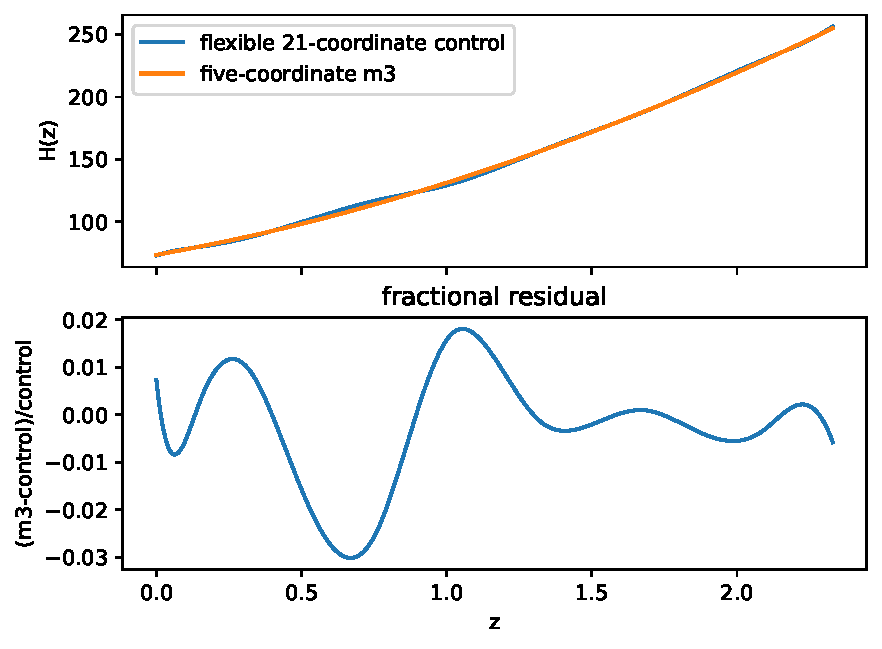
\includegraphics[width=0.9\linewidth]{figures/generated/bridge_fig2_m3}
  \caption{Five-coordinate order-3 reconstruction compared with the
  flexible 21-coordinate control. The lower panel shows
  $(H_{m=3}-H_{\rm control})/H_{\rm control}$.}
  \label{fig:reconstruction-m3}
\end{figure}

\subsection{Predictive validation and the failed continuation}

Orders above the selected $m=3$ model do not provide enough held-out improvement to overcome the predeclared parsimony rule, and still higher orders degrade predictive performance
(Table~\ref{tab:constrained-cv}). The null reconstruction is the undeformed
$\Lambda$CDM reference with zero fitted reconstruction coordinates ($K_{H}$
fixed to no deformation, $\epsilon$ not applicable) and a single
common $M$ profiled per fold-train (null contract,
\path{paper/evidence/likelihood/null_model_contract.json}).
Against this null on identical folds,
the fixed $m=3$ map improves held-out supernova prediction by
$\Delta\chi^{2}=\BridgeNullSn{}$ and improves constrained DESI
($z\le1.8$) by $\Delta\chi^{2}=\BridgeNullDesiConstr{}$ (null reconstruction
$\chi^{2}=\BridgeDesiBareConstr{}$ against
$m=3$ $\chi^{2}=\BridgeDesiMThreeConstr{}$); the order-3 reconstruction fails its $z=2.33$ Ly$\alpha$ continuation test strongly. The Ly$\alpha$ block
is then scored as an out-of-domain continuation test, where every
order shows a large continuation error (Ly$\alpha$ column of
Table~\ref{tab:constrained-cv}). The order-3 continuation
fails, and therefore the reconstruction's constrained domain ends at
$z\le1.8$; this bounds the claim rather than rescuing the model.

\subsection{Statistical interpretation of model selection}
\label{sec:prosecution}

A parametric bootstrap of the entire constrained-domain selection
pipeline under the null reconstruction (250 replicates; same null/candidate
family, data split, bounds and selection rule;
constrained
bootstrap \texttt{bootstrap.json} in paper
evidence)
gives $P(\mathrm{select} \ge m{=}3 \mid \mathrm{null}) =
\CvConstrBootProb{}$, reported exactly as obtained with no threshold
tuning. The Ly$\alpha$ continuation-failure statistic is recorded separately
and never chooses $m$. This bootstrap tests the complexity of the
selected representation, not the existence of the numerical difference
between fixed endpoint histories. Model-order selection alone is not
evidence of a discovery. The reference-sensitivity analysis is a
separate robustness check, not a significance test. The result is presented as a compact reconstruction
with demonstrated held-out behavior.

\begin{figure}[!htbp]
  \centering
  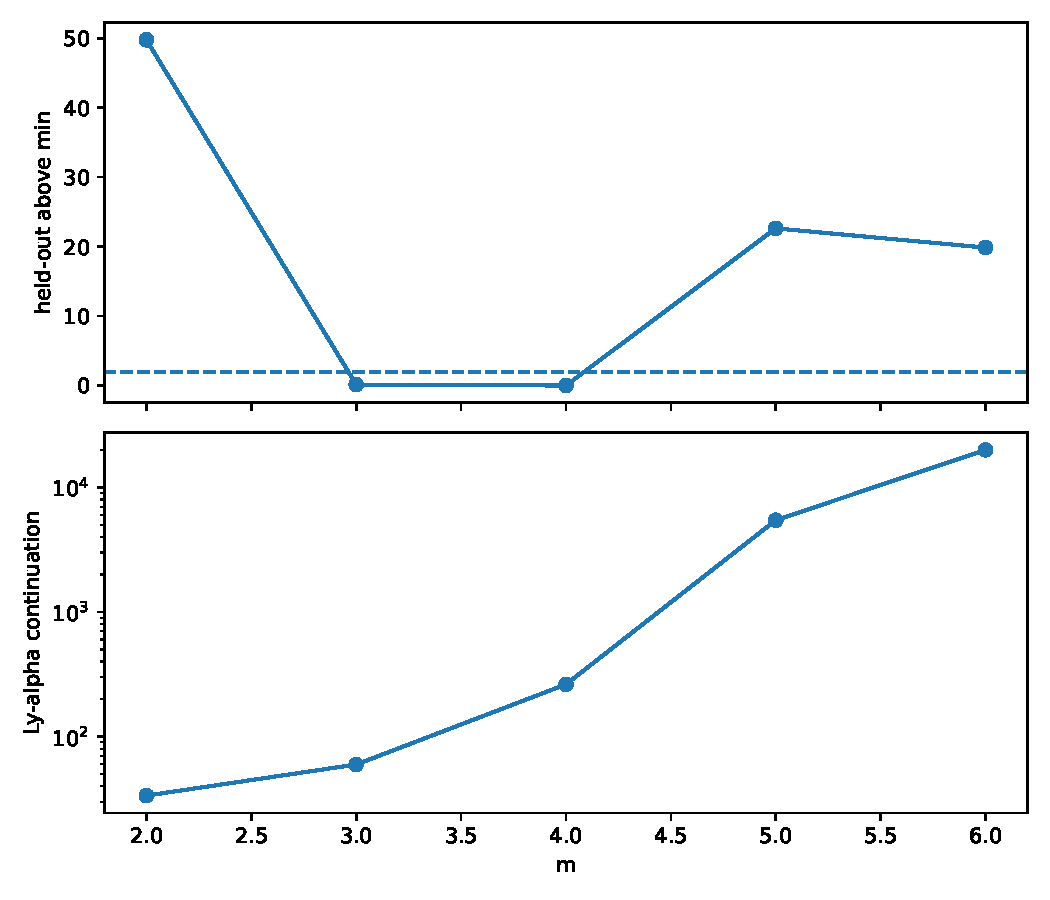
\includegraphics[width=0.9\linewidth]{figures/generated/bridge_fig3_cv}
  \caption{Constrained predictive model selection: held-out
  $\Delta\chi^{2}$ versus the constrained minimum (top; SN plus DESI
  $z\le1.8$), with the Ly$\alpha$ continuation failure on a
  logarithmic scale (bottom; not used in selection). The $m=3$/$m=4$
  near-tie is visible; the dashed line is the within-2 selection
  threshold above the minimum, and the predeclared smallest-$m$-within-2.0 rule
  selects $m=3$.}
  \label{fig:reconstruction-cv}
\end{figure}

\subsection{Reciprocity test}

The ruler/clock split is consistent with zero: $\Delta\chi^{2}
(\epsilon{=}0)=\BridgeEpsDelta{}$, with 1-sigma profile
approximately $[-0.012,+0.005]$. No nonreciprocal calibration is
detected; $\epsilon$ is not detected.

\begin{figure}[!htbp]
  \centering
  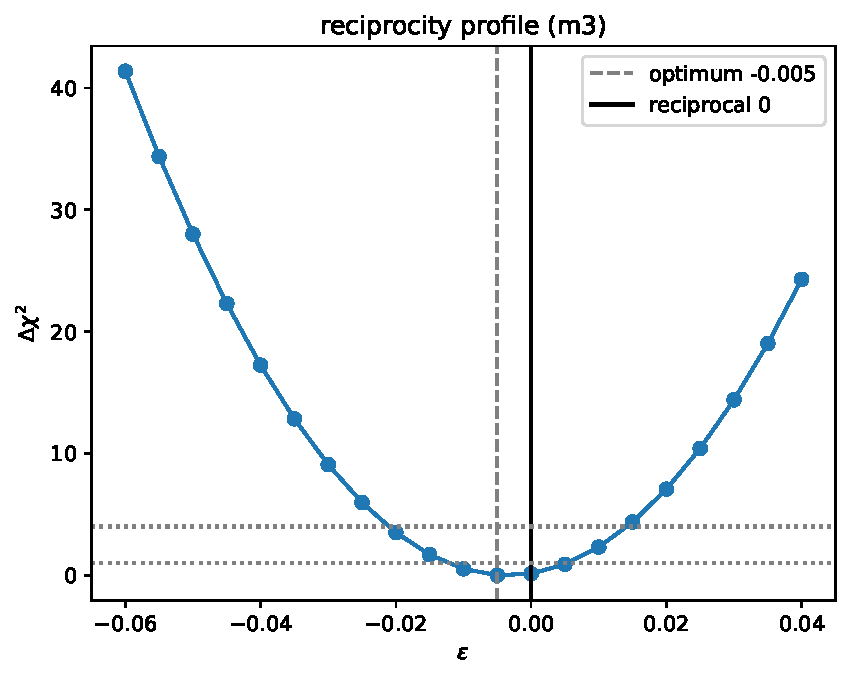
\includegraphics[width=0.9\linewidth]{figures/generated/bridge_fig4_epsilon}
  \caption{Reciprocity profile $\Delta\chi^{2}(\epsilon)$ in the
  selected $m=3$ map: optimum near $-0.005$ and zero at
  $\Delta\chi^{2}=\BridgeEpsDelta{}$, with horizontal
  $\Delta\chi^{2}=1$ and $4$ levels.}
  \label{fig:reconstruction-epsilon}
\end{figure}

\subsection{Why increased flexibility is rejected}
\label{sec:diagnostic-alternatives}

The analysis actively rejected better-looking training solutions. The
roughness family reaches $\chi^{2}=1453.34$ but its leading shape
coefficient sits exactly at the imposed bound ($c_{1}=+0.5$) with
the local descent gradient pointing outward, so its optimum depends
on the box: it is boundary-limited and retained as a supporting
basis only. The Legendre $m=6$ map reaches good training
$\chi^{2}=1455.19$ with an interior optimum but fails the held-out
Lyman-alpha continuation test (Table~\ref{tab:constrained-cv});
it is therefore not promoted.
Both are retained as fixed diagnostic alternatives in
evidence.
